\subsubsection{Eliminaci\'on Gaussiana vs Factorizaci\'on de Cholesky (complejidad algor\'timica)}

\textbf{Hip\'otesis:} Tanto el algoritmo de Eliminaci\'on Gaussiana como el de Factorizaci\'on de Cholesky tienen complejidad $O(n^{3})$.


Para analizar la hip\'otesis generamos instancias de posibles partidos de distinta cantidad de jugadores (50, 100, 150... 500). Vamos a tomar n\'umeros aleatorios para seleccionar los equipos y resultados de cada partido y mediremos los tiempos para el algoritmo de Cholesky y el de Eliminaci\'on Gaussiana para cada una de esas instancias de partidos. Para la medici\'on de cada una de estas instancias ejecutamos 40 veces cada algoritmo y registramos el promedio.

El gr\'afico siguiente muestra la cantidad de ticks en promedio (siguiendo el procedimiento mencionado) mostrando una complejidad polinomial del algoritmo.


\begin{figure}[h!]
  \begin{center}
	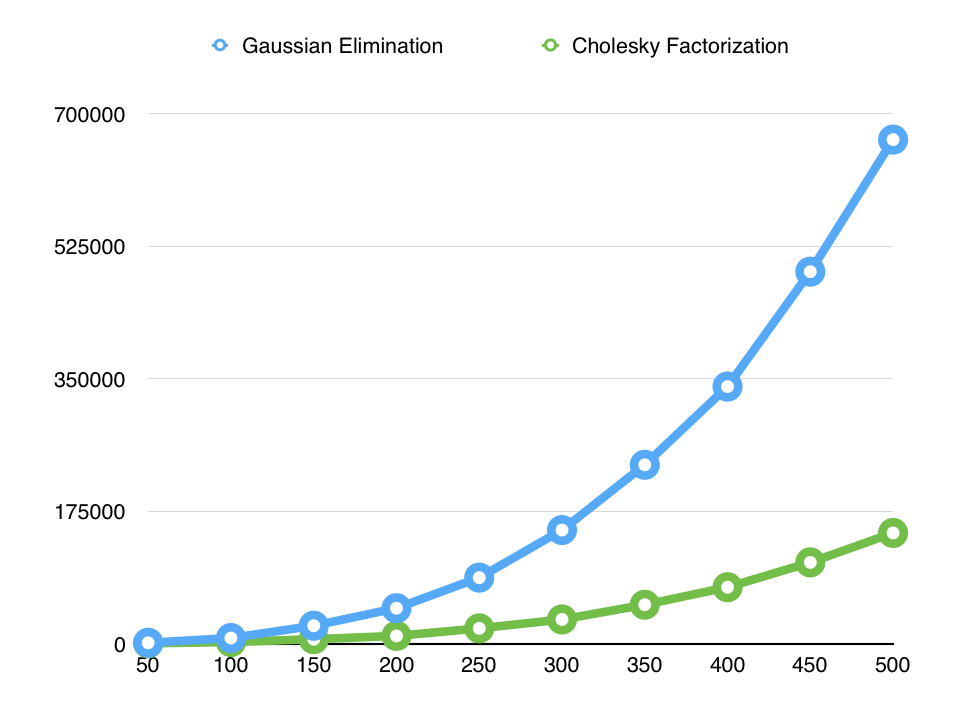
\includegraphics[scale=0.70]{imagenes/cuantitative/default/default1.png}
	\caption{Eliminaci\'on gaussiana vs Factorizaci\'on de Cholesky}
%	\label{bChange}
  \end{center}
\end{figure}

Si a estas funciones las calculamos dividi\'endolas por $n^{2}$ vemos que se obtienen funciones lineales como muestra el siguiente gr\'afico.

\begin{figure}[h!]
  \begin{center}
	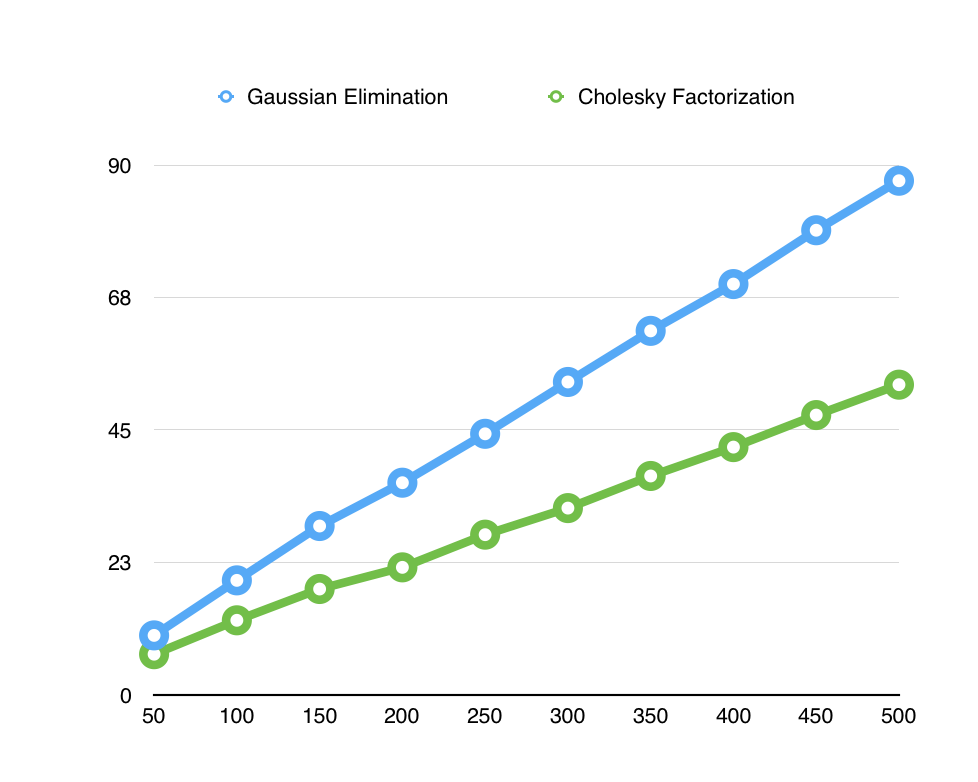
\includegraphics[scale=0.70]{imagenes/cuantitative/default/default2.png}
	\caption{Eliminaci\'on gaussiana vs Factorizaci\'on de Cholesky (base c\'ubica)}
%	\label{bChange}
  \end{center}
\end{figure}
\newpage

Para concluir que el orden es realmente c\'ubico, tomamos estos mismos datos pero los representamos dividi\'endolos por $n^{3}$. Las funciones que obtenemos vemos que son casi constantes y se estabilizan a medida que n crece. Las instancias de $n$ pequeños tienen una cantidad de ticks levemente mayor pero esto es atribuible a motivos de cach\'e del procesador y procesos paralelos.

\begin{figure}[h!]
  \begin{center}
	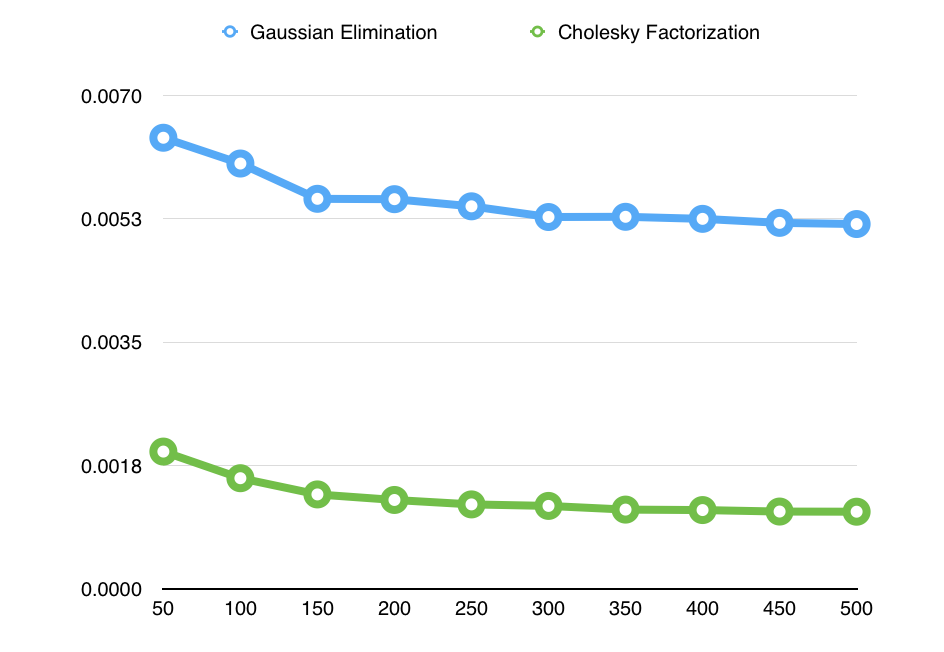
\includegraphics[scale=0.70]{imagenes/cuantitative/default/default3.png}
	\caption{Eliminaci\'on gaussiana vs Factorizaci\'on de Cholesky (base c\'ubica)}
%	\label{bChange}
  \end{center}
\end{figure}
\newpage